\chapter{Analisis}
\label{chap:analisis}

Bab ini membahas tentang cara kerja algoritma \textit{backtracking} dan algoritma \textit{hybrid genetic} untuk menyelesaikan permainan teka-teki Calcudoku.

\section{Algoritma \textit{Backtracking}}
\label{sec:analisisbt}

Untuk mengilustrasikan cara kerja algoritma \textit{backtracking}, akan digunakan permainan teka-teki Calcudoku yang digambarkan pada Gambar~\ref{fig:analisisbt1} sebagai contoh.

\begin{figure}
\centering
\captionsetup{justification=centering}
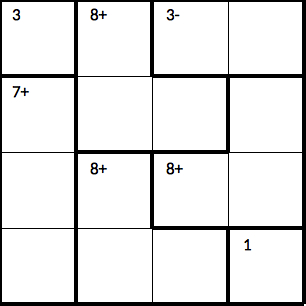
\includegraphics[scale=0.333]{Gambar/backtracking/State1}
\caption[Contoh permainan teka-teki Calcudoku dengan ukuran \textit{grid} 4 x 4 yang belum diselesaikan, seperti yang digambarkan pada Gambar~\ref{fig:backtracking1}.  ~\cite{fahda:16:backtracking}]{Contoh permainan teka-teki dengan ukuran \textit{grid} 4 x 4 yang belum diselesaikan, seperti yang digambarkan pada Gambar~\ref{fig:backtracking1}.  ~\cite{fahda:16:backtracking}}
\label{fig:analisisbt1}
\end{figure}

\begin{enumerate}
\item Algoritma \textit{backtracking} dimulai dengan teka-teki yang belum diselesaikan, seperti yang digambarkan pada Gambar~\ref{fig:analisisbt1} (\textit{state} 1).
\item Algoritma mengisikan sel pada baris ke-1 dan kolom ke-1 dengan angka 1 (\textit{state} 2), tetapi angka 1 tidak sesuai dengan angka tujuan dari \textit{cage} tersebut.
\item Algoritma lalu mencoba kemungkinan angka berikutnya, yaitu angka 2 (\textit{state} 3), tetapi angka 2 juga tidak sesuai dengan angka tujuan dari \textit{cage} tersebut.
\item Algoritma lalu mencoba kemungkinan angka berikutnya, yaitu angka 3 (\textit{state} 4), seperti dapat dilihat pada Gambar~\ref{fig:analisisbt2}, dan ternyata angka 3 sesuai dengan angka tujuan dari \textit{cage} tersebut, sehingga algoritma dapat maju ke sel berikutnya.

\begin{figure}
\centering
\captionsetup{justification=centering}
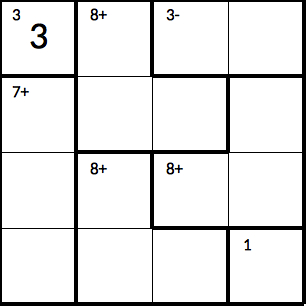
\includegraphics[scale=0.333]{Gambar/backtracking/State4}
\caption[\textit{State} 4]{\textit{State} 4}
\label{fig:analisisbt2}
\end{figure}

\item Algoritma lalu mengisikan sel pada baris ke-1 dan kolom ke-2 dengan angka 1 (\textit{state} 5). Algoritma lalu maju ke sel berikutnya.
\item Algoritma lalu mengisikan sel pada baris ke-1 dan kolom ke-3 dengan angka 1 (\textit{state} 6), tetapi angka 1 sudah pernah digunakan dalam baris tersebut.
\item Algoritma lalu mencoba kemungkinan angka berikutnya, yaitu angka 2 (\textit{state} 7). Algoritma lalu maju ke sel berikutnya.
\item Algoritma lalu mengisikan sel pada baris ke-1 dan kolom ke-4 dengan angka 1 (\textit{state} 8), tetapi angka 1 sudah pernah digunakan dalam baris tersebut.
\item Algoritma lalu mencoba kemungkinan angka berikutnya, yaitu angka 2 (\textit{state} 9), tetapi angka 2 sudah pernah digunakan dalam baris tersebut.
\item Algoritma lalu mencoba kemungkinan angka berikutnya, yaitu angka 3 (\textit{state} 10), tetapi angka 3 sudah pernah digunakan dalam baris tersebut.
\item Algoritma lalu mencoba kemungkinan angka berikutnya, yaitu angka 4 (\textit{state} 11), seperti dapat dilihat pada Gambar~\ref{fig:analisisbt3}, tetapi hasilnya tidak sesuai dengan angka tujuan dari \textit{cage} tersebut.

\begin{figure}
\centering
\captionsetup{justification=centering}
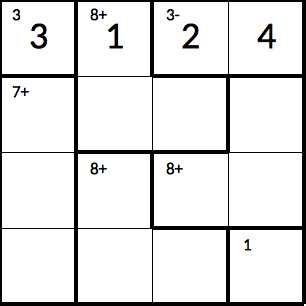
\includegraphics[scale=0.333]{Gambar/backtracking/State11}
\caption[\textit{State} 11]{\textit{State} 11}
\label{fig:analisisbt3}
\end{figure}

\item Karena semua kemungkinan angka untuk baris ke-1 dan kolom ke-4 telah dicoba dan gagal, maka algoritma harus mundur kembali ke (\textit{state} 7). Algoritma mencoba kemungkinan angka berikutnya, yaitu angka 3  (\textit{state} 12), seperti dapat dilihat pada Gambar~\ref{fig:analisisbt4}, tetapi angka 3 sudah pernah digunakan dalam baris tersebut. Algoritma lalu maju ke sel berikutnya.

\begin{figure}
\centering
\captionsetup{justification=centering}
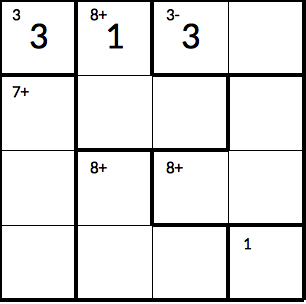
\includegraphics[scale=0.333]{Gambar/backtracking/State12}
\caption[\textit{State} 12]{\textit{State} 12}
\label{fig:analisisbt4}
\end{figure}

\item Algoritma lalu mencoba kemungkinan angka berikutnya, yaitu angka 4 (\textit{state} 13). Algoritma lalu maju ke sel berikutnya.
\item Algoritma lalu mengisikan sel pada baris ke-1 dan kolom ke-4 dengan angka 1 (\textit{state} 14), tetapi angka 1 sudah pernah digunakan dalam baris tersebut.
\item Algoritma lalu mencoba kemungkinan angka berikutnya, yaitu angka 2 (\textit{state} 15), tetapi hasilnya tidak sesuai dengan angka tujuan dari \textit{cage} tersebut.
\item Algoritma lalu mencoba kemungkinan angka berikutnya, yaitu angka 3 (\textit{state} 16), tetapi angka 3 sudah pernah digunakan dalam baris tersebut.
\item Algoritma lalu mencoba kemungkinan angka berikutnya, yaitu angka 4 (\textit{state} 17), seperti dapat dilihat pada Gambar~\ref{fig:analisisbt5}, tetapi angka 4 sudah pernah digunakan dalam baris tersebut.

\begin{figure}
\centering
\captionsetup{justification=centering}
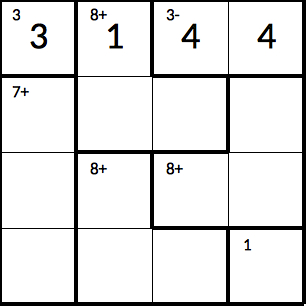
\includegraphics[scale=0.333]{Gambar/backtracking/State17}
\caption[\textit{State} 17]{\textit{State} 17}
\label{fig:analisisbt5}
\end{figure}

\item Karena semua kemungkinan angka untuk baris ke-1 dan kolom ke-3 dan ke-4 telah dicoba dan gagal, maka algoritma harus mundur kembali ke (\textit{state} 5). Algoritma mencoba kemungkinan angka berikutnya, yaitu angka 2  (\textit{state} 18), seperti dapat dilihat pada Gambar~\ref{fig:analisisbt6}. Algoritma lalu maju ke sel berikutnya.

\begin{figure}
\centering
\captionsetup{justification=centering}
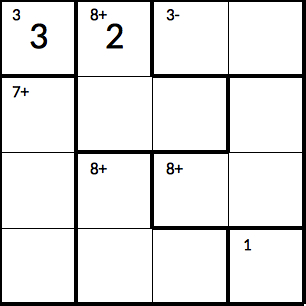
\includegraphics[scale=0.333]{Gambar/backtracking/State18}
\caption[\textit{State} 18]{\textit{State} 18}
\label{fig:analisisbt6}
\end{figure}

\item Algoritma lalu mengisikan sel pada baris ke-1 dan kolom ke-3 dengan angka 1 (\textit{state} 19), seperti dapat dilihat pada Gambar~\ref{fig:analisisbt7}. Algoritma lalu maju ke sel berikutnya.

\begin{figure}
\centering
\captionsetup{justification=centering}
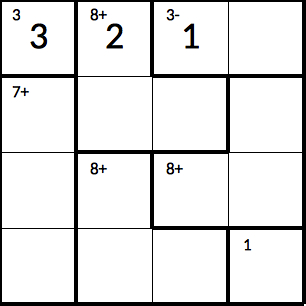
\includegraphics[scale=0.333]{Gambar/backtracking/State19}
\caption[\textit{State} 19]{\textit{State} 19}
\label{fig:analisisbt7}
\end{figure}

\item Algoritma lalu mengisikan sel pada baris ke-1 dan kolom ke-4 dengan angka 1 (\textit{state} 20), tetapi angka 1 sudah pernah digunakan dalam baris tersebut.
\item Algoritma lalu mencoba kemungkinan angka berikutnya, yaitu angka 2 (\textit{state} 21), tetapi angka 2 sudah pernah digunakan dalam baris tersebut.
\item Algoritma lalu mencoba kemungkinan angka berikutnya, yaitu angka 3 (\textit{state} 22), tetapi angka 3 sudah pernah digunakan dalam baris tersebut.
\item Algoritma lalu mencoba kemungkinan angka berikutnya, yaitu angka 4 (\textit{state} 23), dan ternyata hasilnya sesuai dengan angka tujuan dari \textit{cage} tersebut, seperti dapat dilihat pada Gambar~\ref{fig:analisisbt8}. Algoritma telah selesai mengisikan baris ke-1, sehingga bisa maju ke baris berikutnya.

\begin{figure}
\centering
\captionsetup{justification=centering}
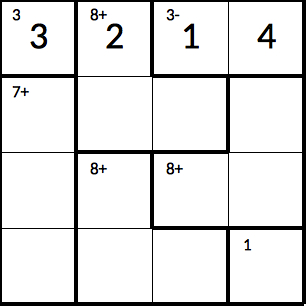
\includegraphics[scale=0.333]{Gambar/backtracking/State23}
\caption[\textit{State} 23]{\textit{State} 23}
\label{fig:analisisbt8}
\end{figure}

\item Algoritma lalu mengisikan sel pada baris ke-2 dan kolom ke-1 dengan angka 1 (\textit{state} 24), seperti dapat dilihat pada Gambar~\ref{fig:analisisbt9}. Algoritma lalu maju ke sel berikutnya.

\begin{figure}
\centering
\captionsetup{justification=centering}
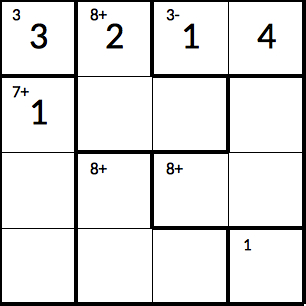
\includegraphics[scale=0.333]{Gambar/backtracking/State24}
\caption[\textit{State} 24]{\textit{State} 24}
\label{fig:analisisbt9}
\end{figure}

\item Algoritma lalu mengisikan sel pada baris ke-2 dan kolom ke-2 dengan angka 1 (\textit{state} 25), tetapi angka 1 sudah pernah digunakan dalam baris tersebut.
\item Algoritma lalu mencoba kemungkinan angka berikutnya, yaitu angka 2 (\textit{state} 26), tetapi angka 2 sudah pernah digunakan dalam kolom tersebut.
\item Algoritma lalu mencoba kemungkinan angka berikutnya, yaitu angka 3 (\textit{state} 27). Algoritma lalu maju ke sel berikutnya.
\item Algoritma lalu mengisikan sel pada baris ke-2 dan kolom ke-3 dengan angka 1 (\textit{state} 28), tetapi angka 1 sudah pernah digunakan dalam baris dan kolom tersebut.
\item Algoritma lalu mencoba kemungkinan angka berikutnya, yaitu angka 2 (\textit{state} 29), tetapi hasilnya tidak sesuai dengan angka tujuan dari \textit{cage} tersebut.
\item Algoritma lalu mencoba kemungkinan angka berikutnya, yaitu angka 3 (\textit{state} 30), tetapi angka 3 sudah pernah digunakan dalam baris tersebut.
\item Algoritma lalu mencoba kemungkinan angka berikutnya, yaitu angka 4 (\textit{state} 31), seperti dapat dilihat pada Gambar~\ref{fig:analisisbt10}, tetapi hasilnya tidak sesuai dengan angka tujuan dari \textit{cage} tersebut.

\begin{figure}
\centering
\captionsetup{justification=centering}
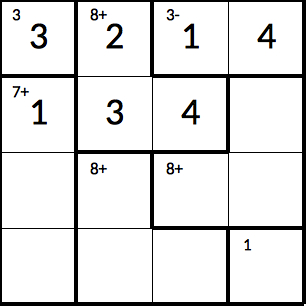
\includegraphics[scale=0.333]{Gambar/backtracking/State31}
\caption[\textit{State} 31]{\textit{State} 31}
\label{fig:analisisbt10}
\end{figure}

\item Karena semua kemungkinan angka untuk baris ke-2 dan kolom ke-3 telah dicoba dan gagal, maka algoritma harus mundur kembali ke (\textit{state} 27). Algoritma mencoba kemungkinan angka berikutnya, yaitu angka 4 (\textit{state} 32), seperti dapat dilihat pada Gambar~\ref{fig:analisisbt11}. Algoritma lalu maju ke sel berikutnya.

\begin{figure}
\centering
\captionsetup{justification=centering}
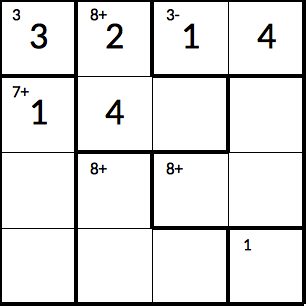
\includegraphics[scale=0.333]{Gambar/backtracking/State32}
\caption[\textit{State} 32]{\textit{State} 32}
\label{fig:analisisbt11}
\end{figure}

\item Algoritma lalu mengisikan sel pada baris ke-2 dan kolom ke-3 dengan angka 1 (\textit{state} 33), tetapi angka 1 sudah pernah digunakan dalam baris tersebut.
\item Algoritma lalu mencoba kemungkinan angka berikutnya, yaitu angka 2 (\textit{state} 34), dan ternyata hasilnya sesuai dengan angka tujuan dari \textit{cage} tersebut, seperti dapat dilihat pada Gambar~\ref{fig:analisisbt12}. Algoritma lalu maju ke sel berikutnya.

\begin{figure}
\centering
\captionsetup{justification=centering}
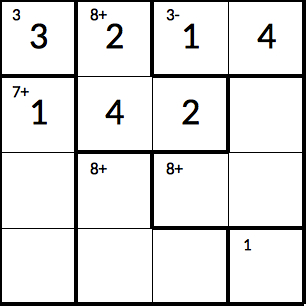
\includegraphics[scale=0.333]{Gambar/backtracking/State34}
\caption[\textit{State} 34]{\textit{State} 34}
\label{fig:analisisbt12}
\end{figure}

\item Algoritma lalu mengisikan sel pada baris ke-2 dan kolom ke-4 dengan angka 1 (\textit{state} 35), tetapi angka 1 sudah pernah digunakan dalam baris tersebut.
\item Algoritma lalu mencoba kemungkinan angka berikutnya, yaitu angka 2 (\textit{state} 36), tetapi angka 2 sudah pernah digunakan dalam baris tersebut.
\item Algoritma lalu mencoba kemungkinan angka berikutnya, yaitu angka 3 (\textit{state} 37), seperti dapat dilihat pada Gambar~\ref{fig:analisisbt13}. Algoritma telah selesai mengisikan baris ke-2, sehingga bisa maju ke baris berikutnya.

\begin{figure}
\centering
\captionsetup{justification=centering}
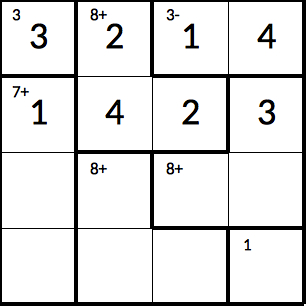
\includegraphics[scale=0.333]{Gambar/backtracking/State37}
\caption[\textit{State} 37]{\textit{State} 37}
\label{fig:analisisbt13}
\end{figure}

\item Algoritma lalu mengisikan sel pada baris ke-3 dan kolom ke-1 dengan angka 1 (\textit{state} 38), tetapi angka 1 sudah pernah digunakan dalam kolom tersebut.
\item Algoritma lalu mencoba kemungkinan angka berikutnya, yaitu angka 2 (\textit{state} 39). Algoritma lalu maju ke sel berikutnya.
\item Algoritma lalu mengisikan sel pada baris ke-3 dan kolom ke-2 dengan angka 1 (\textit{state} 40). Algoritma lalu maju ke sel berikutnya.
\item Algoritma lalu mengisikan sel pada baris ke-3 dan kolom ke-3 dengan angka 1 (\textit{state} 41), tetapi angka 1 sudah pernah digunakan dalam baris dan kolom tersebut.
\item Algoritma lalu mencoba kemungkinan angka berikutnya, yaitu angka 2 (\textit{state} 42), tetapi angka 2 sudah pernah digunakan dalam baris dan kolom tersebut.
\item Algoritma lalu mencoba kemungkinan angka berikutnya, yaitu angka 3 (\textit{state} 43). Algoritma lalu maju ke sel berikutnya.
\item Algoritma lalu mengisikan sel pada baris ke-3 dan kolom ke-4 dengan angka 1 (\textit{state} 44), tetapi angka 1 sudah pernah digunakan dalam baris tersebut.
\item Algoritma lalu mencoba kemungkinan angka berikutnya, yaitu angka 2 (\textit{state} 45), tetapi angka 2 sudah pernah digunakan dalam baris tersebut.
\item Algoritma lalu mencoba kemungkinan angka berikutnya, yaitu angka 3 (\textit{state} 46), tetapi angka 3 sudah pernah digunakan dalam baris dan kolom tersebut.
\item Algoritma lalu mencoba kemungkinan angka berikutnya, yaitu angka 4 (\textit{state} 47), seperti dapat dilihat pada Gambar~\ref{fig:analisisbt14}, tetapi hasilnya tidak sesuai dengan angka tujuan dari \textit{cage} tersebut.

\begin{figure}
\centering
\captionsetup{justification=centering}
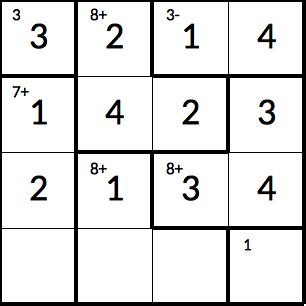
\includegraphics[scale=0.333]{Gambar/backtracking/State47}
\caption[\textit{State} 47]{\textit{State} 47}
\label{fig:analisisbt14}
\end{figure}

\item Karena semua kemungkinan angka untuk baris ke-3 dan kolom ke-4 telah dicoba dan gagal, maka algoritma harus mundur kembali ke (\textit{state} 43). Algoritma lalu mencoba kemungkinan angka berikutnya, yaitu angka 4 (\textit{state} 48), seperti dapat dilihat pada Gambar~\ref{fig:analisisbt15}. Algoritma lalu maju ke sel berikutnya.

\begin{figure}
\centering
\captionsetup{justification=centering}
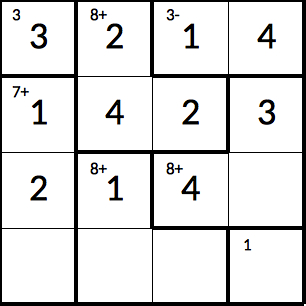
\includegraphics[scale=0.333]{Gambar/backtracking/State48}
\caption[\textit{State} 48]{\textit{State} 48}
\label{fig:analisisbt15}
\end{figure}

\item Algoritma lalu mengisikan sel pada baris ke-3 dan kolom ke-4 dengan angka 1 (\textit{state} 49), tetapi angka 1 sudah pernah digunakan dalam baris tersebut.
\item Algoritma lalu mencoba kemungkinan angka berikutnya, yaitu angka 2 (\textit{state} 50), tetapi angka 2 sudah pernah digunakan dalam baris tersebut.
\item Algoritma lalu mencoba kemungkinan angka berikutnya, yaitu angka 3 (\textit{state} 51), tetapi angka 3 sudah pernah digunakan dalam kolom tersebut.
\item Algoritma lalu mencoba kemungkinan angka berikutnya, yaitu angka 4 (\textit{state} 52), seperti dapat dilihat pada Gambar~\ref{fig:analisisbt16}, tetapi angka 3 sudah pernah digunakan dalam baris dan kolom tersebut.

\begin{figure}
\centering
\captionsetup{justification=centering}
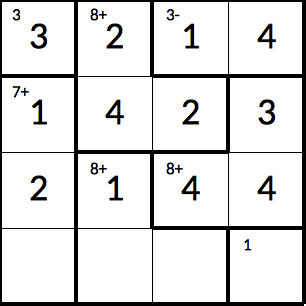
\includegraphics[scale=0.333]{Gambar/backtracking/State52}
\caption[\textit{State} 52]{\textit{State} 52}
\label{fig:analisisbt16}
\end{figure}

\item Karena semua kemungkinan angka untuk baris ke-3 dan kolom ke-4 telah dicoba dan gagal, maka algoritma harus mundur kembali ke (\textit{state} 48). Algoritma lalu mencoba kemungkinan angka berikutnya, yaitu angka 2 (\textit{state} 53) seperti dapat dilihat pada Gambar~\ref{fig:analisisbt17}, tetapi angka 2 sudah pernah digunakan dalam baris dan kolom tersebut.

\begin{figure}
\centering
\captionsetup{justification=centering}
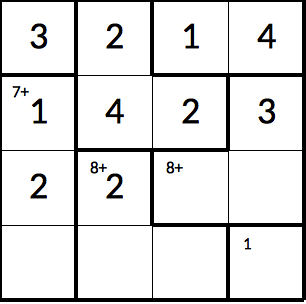
\includegraphics[scale=0.333]{Gambar/backtracking/State53}
\caption[\textit{State} 53]{\textit{State} 53}
\label{fig:analisisbt17}
\end{figure}

\item Algoritma lalu mencoba kemungkinan angka berikutnya, yaitu angka 3 (\textit{state} 54). Algoritma lalu maju ke sel berikutnya.
\item Algoritma lalu mengisikan sel pada baris ke-3 dan kolom ke-3 dengan angka 1 (\textit{state} 55), tetapi angka 1 sudah pernah digunakan dalam kolom tersebut.
\item Algoritma lalu mencoba kemungkinan angka berikutnya, yaitu angka 2 (\textit{state} 56), tetapi angka 2 sudah pernah digunakan dalam baris dan kolom tersebut.
\item Algoritma lalu mencoba kemungkinan angka berikutnya, yaitu angka 3 (\textit{state} 57), tetapi angka 3 sudah pernah digunakan dalam baris tersebut.
\item Algoritma lalu mencoba kemungkinan angka berikutnya, yaitu angka 4 (\textit{state} 58). Algoritma lalu maju ke sel berikutnya.
\item Algoritma lalu mengisikan sel pada baris ke-3 dan kolom ke-4 dengan angka 1 (\textit{state} 59). Algoritma telah selesai mengisikan baris ke-2, sehingga bisa maju ke baris berikutnya.
\item Algoritma lalu mengisikan sel pada baris ke-4 dan kolom ke-1 dengan angka 1 (\textit{state} 60), tetapi angka 1 sudah pernah digunakan dalam kolom tersebut.
\item Algoritma lalu mencoba kemungkinan angka berikutnya, yaitu angka 2 (\textit{state} 61), tetapi angka 2 sudah pernah digunakan dalam kolom tersebut.
\item Algoritma lalu mencoba kemungkinan angka berikutnya, yaitu angka 3 (\textit{state} 62), tetapi angka 3 sudah pernah digunakan dalam kolom tersebut.
\item Algoritma lalu mencoba kemungkinan angka berikutnya, yaitu angka 4 (\textit{state} 63). Algoritma lalu maju ke sel berikutnya.
\item Algoritma lalu mengisikan sel pada baris ke-4 dan kolom ke-2 dengan angka 1 (\textit{state} 64). Algoritma lalu maju ke sel berikutnya.
\item Algoritma lalu mengisikan sel pada baris ke-4 dan kolom ke-3 dengan angka 1 (\textit{state} 65), tetapi angka 1 sudah pernah digunakan dalam baris dan kolom tersebut.
\item Algoritma lalu mencoba kemungkinan angka berikutnya, yaitu angka 2 (\textit{state} 66), tetapi angka 2 sudah pernah digunakan dalam kolom tersebut.
\item Algoritma lalu mencoba kemungkinan angka berikutnya, yaitu angka 3 (\textit{state} 67), tetapi hasilnya tidak sesuai dengan angka tujuan dari \textit{cage} tersebut.
\item Algoritma lalu mencoba kemungkinan angka berikutnya, yaitu angka 4 (\textit{state} 68), seperti dapat dilihat di Gambar~\ref{fig:analisisbt18}. tetapi angka 4 sudah pernah digunakan dalam baris dan kolom tersebut.

\begin{figure}
\centering
\captionsetup{justification=centering}
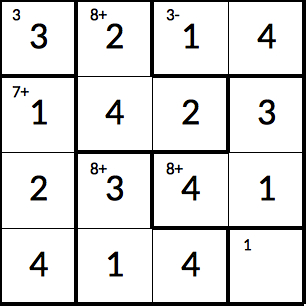
\includegraphics[scale=0.333]{Gambar/backtracking/State68}
\caption[\textit{State} 68]{\textit{State} 68}
\label{fig:analisisbt18}
\end{figure}

\item Karena semua kemungkinan angka untuk baris ke-4 dan kolom ke-3 telah dicoba dan gagal, maka algoritma harus mundur kembali ke (\textit{state} 64). Algoritma lalu mencoba kemungkinan angka berikutnya, yaitu angka 2 (\textit{state} 69), seperti dapat dilihat pada Gambar~\ref{fig:analisisbt19}, tetapi angka 2 sudah pernah digunakan dalam kolom tersebut.

\begin{figure}
\centering
\captionsetup{justification=centering}
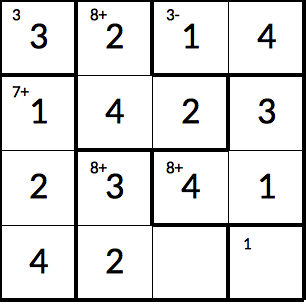
\includegraphics[scale=0.333]{Gambar/backtracking/State69}
\caption[\textit{State} 69]{\textit{State} 69}
\label{fig:analisisbt19}
\end{figure}

\item Algoritma lalu mencoba kemungkinan angka berikutnya, yaitu angka 3 (\textit{state} 70), tetapi angka 3 sudah pernah digunakan dalam kolom tersebut.
\item Algoritma lalu mencoba kemungkinan angka berikutnya, yaitu angka 4 (\textit{state} 71), seperti dapat dilihat di Gambar~\ref{fig:analisisbt20}, tetapi angka 4 sudah pernah digunakan dalam kolom tersebut.

\begin{figure}
\centering
\captionsetup{justification=centering}
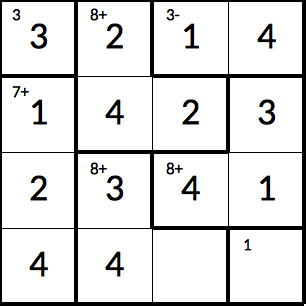
\includegraphics[scale=0.333]{Gambar/backtracking/State71}
\caption[\textit{State} 71]{\textit{State} 71}
\label{fig:analisisbt20}
\end{figure}

\item Karena semua kemungkinan angka untuk baris ke-4 dan kolom ke-1 dan ke-2 telah dicoba dan gagal, maka algoritma harus mundur kembali ke (\textit{state} 59). Algoritma lalu mencoba kemungkinan angka berikutnya, yaitu angka 2 (\textit{state} 72), seperti dapat dilihat pada Gambar~\ref{fig:analisisbt21}, tetapi angka 2 sudah pernah digunakan dalam baris tersebut.

\begin{figure}
\centering
\captionsetup{justification=centering}
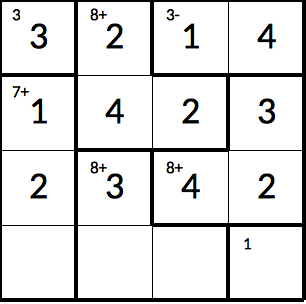
\includegraphics[scale=0.333]{Gambar/backtracking/State72}
\caption[\textit{State} 72]{\textit{State} 72}
\label{fig:analisisbt21}
\end{figure}

\item Algoritma lalu mencoba kemungkinan angka berikutnya, yaitu angka 3 (\textit{state} 73), tetapi angka 3 sudah pernah digunakan dalam baris dan kolom tersebut.
\item Algoritma lalu mencoba kemungkinan angka berikutnya, yaitu angka 4 (\textit{state} 74), seperti dapat dilihat di Gambar~\ref{fig:analisisbt22}, tetapi angka 4 sudah pernah digunakan dalam baris dan kolom tersebut.

\begin{figure}
\centering
\captionsetup{justification=centering}
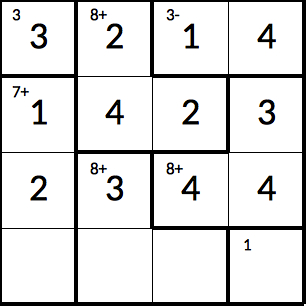
\includegraphics[scale=0.333]{Gambar/backtracking/State74}
\caption[\textit{State} 74]{\textit{State} 74}
\label{fig:analisisbt22}
\end{figure}

\item Karena semua kemungkinan angka untuk baris ke-3 dan kolom ke-3 dan ke-4 telah dicoba dan gagal, maka algoritma harus mundur kembali ke (\textit{state} 54). Algoritma lalu mencoba kemungkinan angka berikutnya, yaitu angka 4 (\textit{state} 75), seperti dapat dilihat pada Gambar~\ref{fig:analisisbt23}, tetapi angka 4 sudah pernah digunakan dalam kolom tersebut.

\begin{figure}
\centering
\captionsetup{justification=centering}
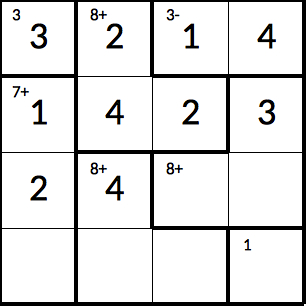
\includegraphics[scale=0.333]{Gambar/backtracking/State75}
\caption[\textit{State} 75]{\textit{State} 75}
\label{fig:analisisbt23}
\end{figure}

\item Karena semua kemungkinan angka untuk baris ke-3 dan kolom ke-2 telah dicoba dan gagal, maka algoritma harus mundur kembali ke (\textit{state} 54). Algoritma lalu mencoba kemungkinan angka berikutnya, yaitu angka 3 (\textit{state} 76), seperti dapat dilihat pada Gambar~\ref{fig:analisisbt24}, tetapi angka 3 sudah pernah digunakan dalam kolom tersebut.

\begin{figure}
\centering
\captionsetup{justification=centering}
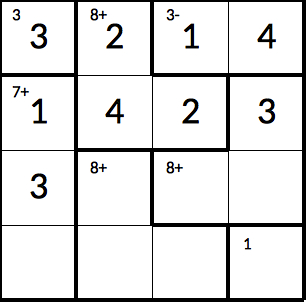
\includegraphics[scale=0.333]{Gambar/backtracking/State76}
\caption[\textit{State} 76]{\textit{State} 76}
\label{fig:analisisbt24}
\end{figure}

\item Algoritma lalu mencoba kemungkinan angka berikutnya, yaitu angka 4 (\textit{state} 77), seperti dapat dilihat di Gambar~\ref{fig:analisisbt25}. Algoritma lalu maju ke sel berikutnya.

\begin{figure}
\centering
\captionsetup{justification=centering}
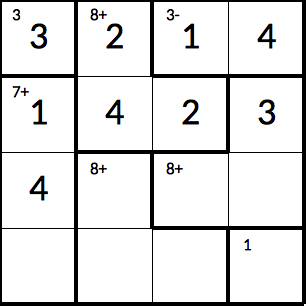
\includegraphics[scale=0.333]{Gambar/backtracking/State77}
\caption[\textit{State} 77]{\textit{State} 77}
\label{fig:analisisbt25}
\end{figure}

\item Algoritma lalu mengisikan sel pada baris ke-3 dan kolom ke-2 dengan angka 1 (\textit{state} 78), seperti dapat dilihat di Gambar~\ref{fig:analisisbt26}. Algoritma lalu maju ke sel berikutnya.

\begin{figure}
\centering
\captionsetup{justification=centering}
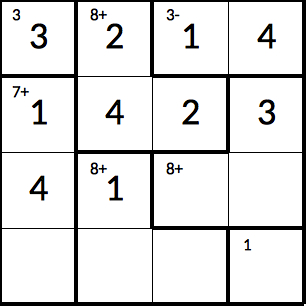
\includegraphics[scale=0.333]{Gambar/backtracking/State78}
\caption[\textit{State} 78]{\textit{State} 78}
\label{fig:analisisbt26}
\end{figure}

\item Algoritma lalu mengisikan sel pada baris ke-3 dan kolom ke-3 dengan angka 1 (\textit{state} 79), tetapi angka 1 sudah pernah digunakan dalam baris dan kolom tersebut.
\item Algoritma lalu mencoba kemungkinan angka berikutnya, yaitu angka 2 (\textit{state} 80), tetapi angka 2 sudah pernah digunakan dalam kolom tersebut.
\item Algoritma lalu mencoba kemungkinan angka berikutnya, yaitu angka 3 (\textit{state} 81), seperti dapat dilihat pada Gambar~\ref{fig:analisisbt27}. Algoritma lalu maju ke sel berikutnya.

\begin{figure}
\centering
\captionsetup{justification=centering}
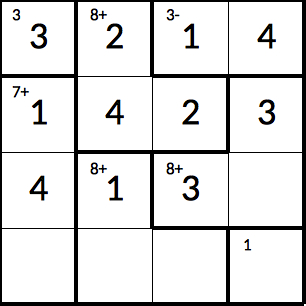
\includegraphics[scale=0.333]{Gambar/backtracking/State81}
\caption[\textit{State} 81]{\textit{State} 81}
\label{fig:analisisbt27}
\end{figure}

\item Algoritma lalu mengisikan sel pada baris ke-3 dan kolom ke-3 dengan angka 1 (\textit{state} 82), tetapi angka 1 sudah pernah digunakan dalam baris tersebut.
\item Algoritma lalu mencoba kemungkinan angka berikutnya, yaitu angka 2 (\textit{state} 83), dan ternyata hasilnya sesuai dengan angka tujuan dari \textit{cage} tersebut, seperti dapat dilihat pada Gambar~\ref{fig:analisisbt28}. Algoritma telah selesai mengisikan baris ke-3, sehingga bisa maju ke baris berikutnya.

\begin{figure}
\centering
\captionsetup{justification=centering}
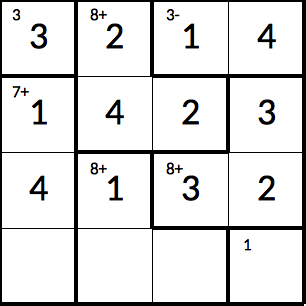
\includegraphics[scale=0.333]{Gambar/backtracking/State83}
\caption[\textit{State} 83]{\textit{State} 83}
\label{fig:analisisbt28}
\end{figure}

\item Algoritma lalu mengisikan sel pada baris ke-4 dan kolom ke-1 dengan angka 1 (\textit{state} 84), tetapi angka 1 sudah pernah digunakan dalam kolom tersebut.
\item Algoritma lalu mencoba kemungkinan angka berikutnya, yaitu angka 2 (\textit{state} 85), dan ternyata hasilnya sesuai dengan angka tujuan dari \textit{cage} tersebut, seperti dapat dilihat pada Gambar~\ref{fig:analisisbt29}. Algoritma lalu maju ke sel berikutnya.

\begin{figure}
\centering
\captionsetup{justification=centering}
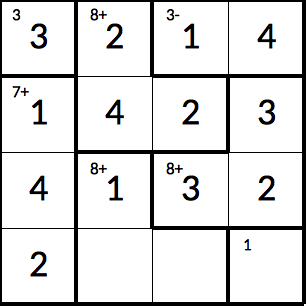
\includegraphics[scale=0.333]{Gambar/backtracking/State85}
\caption[\textit{State} 85]{\textit{State} 85}
\label{fig:analisisbt29}
\end{figure}

\item Algoritma lalu mengisikan sel pada baris ke-4 dan kolom ke-2 dengan angka 1 (\textit{state} 86), tetapi angka 1 sudah pernah digunakan dalam kolom tersebut.
\item Algoritma lalu mencoba kemungkinan angka berikutnya, yaitu angka 2 (\textit{state} 87), tetapi angka 2 sudah pernah digunakan dalam baris dan kolom tersebut.
\item Algoritma lalu mencoba kemungkinan angka berikutnya, yaitu angka 3 (\textit{state} 88), seperti dapat dilihat pada Gambar~\ref{fig:analisisbt30}. Algoritma lalu maju ke sel berikutnya.

\begin{figure}
\centering
\captionsetup{justification=centering}
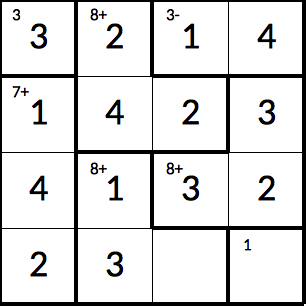
\includegraphics[scale=0.333]{Gambar/backtracking/State88}
\caption[\textit{State} 88]{\textit{State} 88}
\label{fig:analisisbt30}
\end{figure}

\item Algoritma lalu mengisikan sel pada baris ke-4 dan kolom ke-3 dengan angka 1 (\textit{state} 89), tetapi angka 1 sudah pernah digunakan dalam baris dan kolom tersebut.
\item Algoritma lalu mencoba kemungkinan angka berikutnya, yaitu angka 2 (\textit{state} 90), tetapi angka 2 sudah pernah digunakan dalam baris dan kolom tersebut.
\item Algoritma lalu mencoba kemungkinan angka berikutnya, yaitu angka 3 (\textit{state} 91), tetapi angka 3 sudah pernah digunakan dalam kolom tersebut.
\item Algoritma lalu mencoba kemungkinan angka berikutnya, yaitu angka 4 (\textit{state} 92), dan ternyata hasilnya sesuai dengan angka tujuan dari \textit{cage} tersebut, seperti dapat dilihat pada Gambar~\ref{fig:analisisbt31}. Algoritma lalu maju ke sel berikutnya.

\begin{figure}
\centering
\captionsetup{justification=centering}
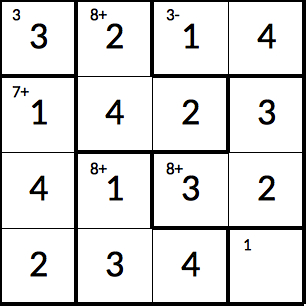
\includegraphics[scale=0.333]{Gambar/backtracking/State92}
\caption[\textit{State} 92]{\textit{State} 92}
\label{fig:analisisbt31}
\end{figure}

\item Algoritma lalu mengisikan sel pada baris ke-4 dan kolom ke-4 dengan angka 1 (\textit{state} 93), dan ternyata hasilnya sesuai dengan angka tujuan dari \textit{cage} tersebut, seperti dapat dilihat pada Gambar~\ref{fig:analisisbt32}. Algoritma \textit{backtracking} telah selesai mengisi semua sel dalam permainan teka-teki Calcudoku ini dengan benar.

\begin{figure}
\centering
\captionsetup{justification=centering}
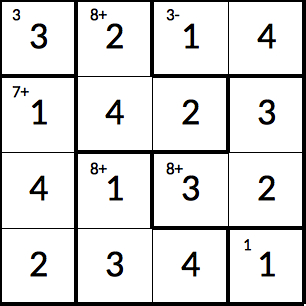
\includegraphics[scale=0.333]{Gambar/backtracking/State93}
\caption[\textit{State} 93]{\textit{State} 93}
\label{fig:analisisbt32}
\end{figure}

\end{enumerate}

Algoritma ini mencapai solusinya pada state 93, seperti pada \textit{state space tree} yang digambarkan dalam Gambar~\ref{fig:analisisbt33}. \textit{State space tree} ini telah mencapai simpul tujuannya, yaitu simpul 93, dengan jalur 3-2-1-4-1-4-2-3-4-1-3-2-2-3-4-1.

\begin{landscape}
\begin{figure}
\centering
\captionsetup{justification=centering}
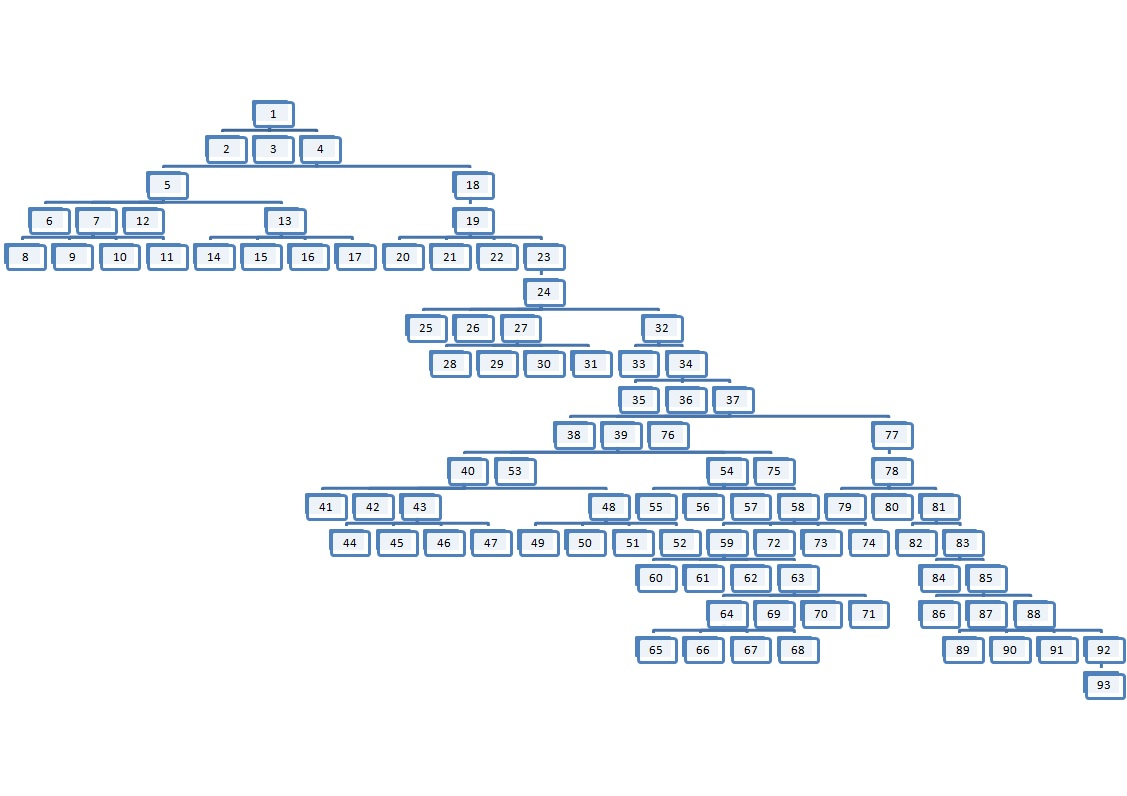
\includegraphics[scale=0.75]{Gambar/backtracking/StateSpaceTree}
\caption[\textit{State space tree} yang dikembangkan dalam proses menyelesaikan teka-teki Calcudoku yang digambarkan pada Gambar~\ref{fig:analisisbt1}]{\textit{State space tree} yang dikembangkan dalam proses menyelesaikan teka-teki Calcudoku yang digambarkan pada Gambar~\ref{fig:analisisbt1}}
\label{fig:analisisbt33}
\end{figure}
\end{landscape}

